\chapter{General Instructions}


The first letter of all \textit{main} words in the chapter heading, section heading etc. must be capitalized. Always have at least 1 paragraph under each header  before the beginning of the next subsection. Make sure that you divide your paragraphs appropriately. A paragraph should not extend for more than three-quarters of a page. All text past this point should be double spaced. 

\section{A word from Dr. G}
Congratulations on reaching this position of starting a thesis. It is indeed a singular achievement and I wish you all the best as you proceed. I wrote this class file as a service to the department and my students. I hope it is of use. I make no claims to the originality of it. It is a combination of original code along with cut and paste snippets from various sources. I recommend you students start a github account and keep updating this class file as you keep making improvements. I do not provide \LaTeX support. But if you ask nicely I am always willing to help, \textit{within reason}, if you stop by my office. Please do not email me with \LaTeX  questions. Again, congratulations and happy writing.

\section{Example Figure}

\begin{figure}[h]
	\centering 
	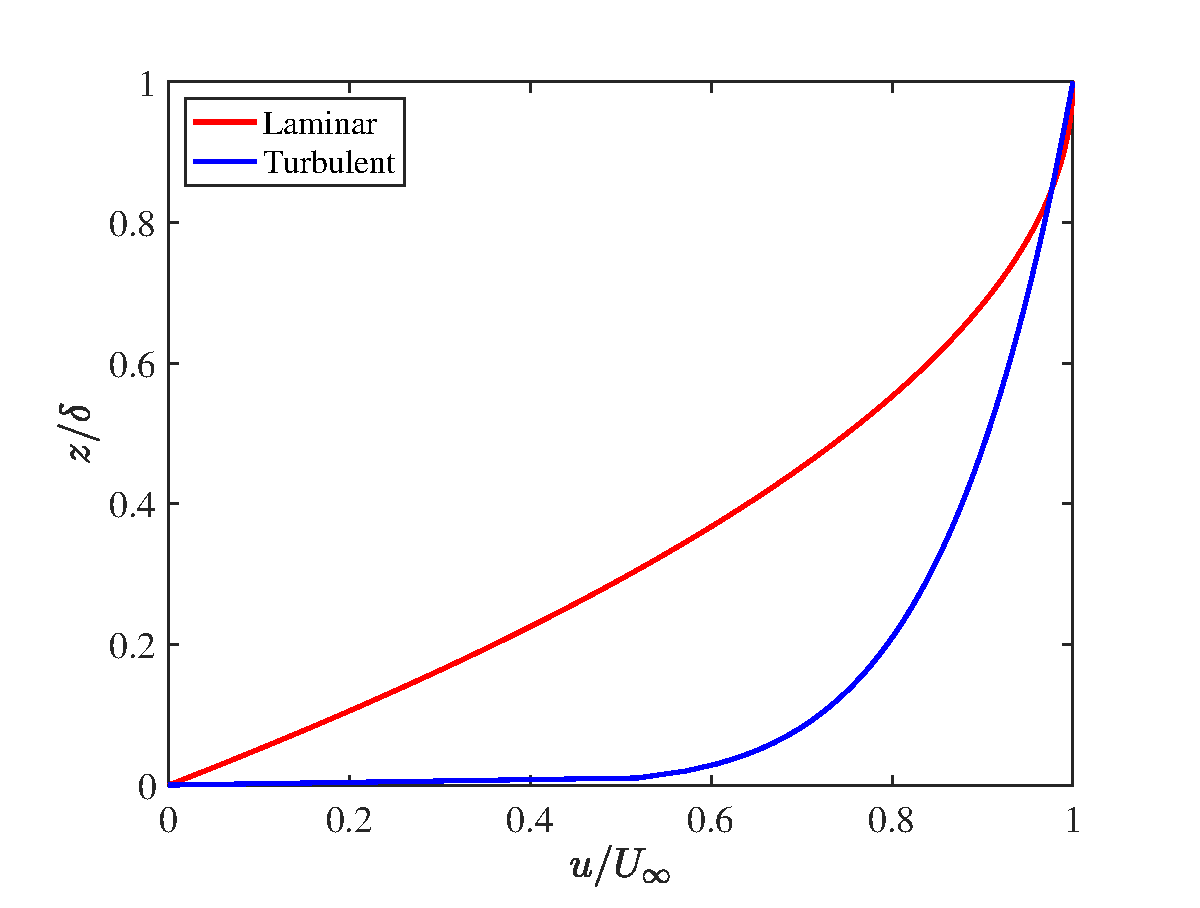
\includegraphics[clip = true,width=0.75\textwidth]{pics/velProf.eps}%
	\caption{Non-dimensional velocity profiles $u/\delta$ corresponding to a laminar and turbulent boundary layer. \nomenclature{\(u\)}{streamwise velocity} \nomenclature{\( \delta\)}{Boundary layer thickness}}
	\label{fg:sampFig1}
\end{figure}

This section will give you a brief example of how to add a figure and automatically cross reference it. Doing it in the following manner will also automatically populate your list of figures. The Figure~\ref{fg:sampFig1} is an example figure. Note, this is in \verb|*.eps| for encapsulated postscript format. The encapsulated postscript format at 300 dpi or greater gives the best print quality. If image size becomes an issue \verb|*.png| is the next best format. The figure caption goes below the figure. Note, the text in the figure is about the same font size as that of the main text. Use the \verb|graphicx| package to insert figures. For sideways figure use the \verb|rotating| package. Please refer to the supplied latex files for a basic example. While referencing a figure in the text the word ``Figure'' should be capitalized.



\section{Example Table}
This section will give you a brief example of how to add a table and automatically cross reference it. A sample table is shown in Table~\ref{tb:sampTab1}. Take advantage of the \verb|tabular| environment. Some other environments to consider are \verb|longtable| and \verb|tabularx|. The caption for a table always goes above the table. Please refer to the supplied latex files for a basic example. While referencing a table in the text the word ``Table'' should be capitalized.

\begin{table}[h]
\centering
\caption{This is a sample table} 
\begin{tabular}{ |l|c|c|c| } 
 \hline \hline
  & case 1 & case 2 & case 3 \\
 \hline \hline
 Parameter 1 ($x$) & 0.345 & 0.434 & 0.55  \\ 
 Parameter 2 ($y$) & 0.345 & 0.434 & 0.55  \\ 
 Parameter 3 ($z$) & 0.345 & 0.434 & 0.55  \\ 
 \hline
\end{tabular}
\label{tb:sampTab1}
\end{table}

\section{Example Equation}

An example of an equations that appears within the body of the text is $p+1/2 \rho V^2=\textrm{constant}$. An example of an equation that is outside the body of the text is

\begin{equation}
    \frac{\partial u}{\partial t} = c\frac{\partial u}{\partial x}
\end{equation}

Some other environments to consider while using equations are \verb|eqnarray| and \verb|align|.
\section{List of Figures, Tables and Nomenclature}
If figures are labelled and captioned appropriately, the List of Figures and Tables should auto-populate. Use the \verb|nomencl| package to automatically populate the nomenclature section. The syntax is \verb|\nomenclature{}{}|. Please refer to the supplied latex files for basic examples. 

\section{Bibliography}
It is the Department of Aerospace Engineering policy that the AIAA Journal format is followed for references. If the \verb|erauAEThesis.cls| file is used, this is built in and no further modifications are needed. Note, references for journal papers (e.g. \citet{Adrian2007a}), conference papers (e.g. \citet{Thompson1989a} ), books (e.g. \citet{Panton2013a}), dissertation/thesis (e.g. \citet{Tseng1983a}) etc. all have specific inputs and formats. Use the command \verb|\citep| for citation only. On the other hand use \verb|\citet| when referencing a citation in the text. For example, \citet{Adrian2007a} (\verb|citet| was used here) is an example of a journal paper while the other kinds of references are books, dissertations, conference proceeding etc. \citep{Panton2013a,Tseng1983a,Thompson1989a} (\verb|citep| was used here).



\nomenclature{\(C_l\)}{ Coefficient of lift}
\nomenclature{\(\alpha\)}{angle of attack}
\nomenclature{\(C_d \)}{Coefficient of drag}
\nomenclature{\(C_m \)}{Moment coefficient}
\nomenclature{\(\tau\)}{shear stress}
\nomenclature{\(C_l\)}{ Coefficient of lift}
\nomenclature{\(\beta\)}{Sweep}
\nomenclature{\(v \)}{spanwise velocity}
\nomenclature{\(w \)}{wall-normal velocity}
\nomenclature{\(p \)}{static pressure}
\nomenclature{\(p_0 \)}{stagnation pressure}
\nomenclature{\(q \)}{dynamic pressure}
\nomenclature{\(M \)}{$={a}/{V_\infty}$ Mach number}
\nomenclature{\(a \)}{Speed of sound}
\nomenclature{\(V_\infty \)}{free-stream velocity}
\nomenclature{\(Re \)}{Reynolds number}
\nomenclature{\(x \)}{streamwise ordinate}
\nomenclature{\(y\)}{spanwise ordinate}
\nomenclature{\(z\)}{wall-normal ordinate}
